%%%%%%%%%%%%%%%%%%%%%%%%%%%%%%%%%%%%%%%%%
% Journal Article
% LaTeX Template
% Version 2.0 (February 7, 2023)
%
% This template originates from:
% https://www.LaTeXTemplates.com
%
% Author:
% Vel (vel@latextemplates.com)
%
% License:
% CC BY-NC-SA 4.0 (https://creativecommons.org/licenses/by-nc-sa/4.0/)
%
% NOTE: The bibliography needs to be compiled using the biber engine.
%
%%%%%%%%%%%%%%%%%%%%%%%%%%%%%%%%%%%%%%%%%

%----------------------------------------------------------------------------------------
%	PACKAGES AND OTHER DOCUMENT CONFIGURATIONS
%----------------------------------------------------------------------------------------

\documentclass[
	a4paper, % Paper size, use either a4paper or letterpaper
	10pt, % Default font size, can also use 11pt or 12pt, although this is not recommended
	unnumberedsections, % Comment to enable section numbering
	twoside, % Two side traditional mode where headers and footers change between odd and even pages, comment this option to make them fixed
]{LTJournalArticle}

\usepackage{hyperref}
\setlength{\parskip}{\baselineskip}%
\setlength{\parindent}{10pt}%
\usepackage{indentfirst}
\usepackage{float}

\addbibresource{References.bib} % BibLaTeX bibliography file

\runninghead{Aquí el titulito} % A shortened article title to appear in the running head, leave this command empty for no running head

\footertext{\textit{}} % Text to appear in the footer, leave this command empty for no footer text

\setcounter{page}{1} % The page number of the first page, set this to a higher number if the article is to be part of an issue or larger work

%----------------------------------------------------------------------------------------
%	TITLE SECTION
%----------------------------------------------------------------------------------------

\title{Luego pienso en el título\\ Va a estar chilero} % Article title, use manual lines breaks (\\) to beautify the layout

% Authors are listed in a comma-separated list with superscript numbers indicating affiliations
% \thanks{} is used for any text that should be placed in a footnote on the first page, such as the corresponding author's email, journal acceptance dates, a copyright/license notice, keywords, etc
\author{%
	Hernández, Giovanna\textsuperscript{1}\thanks{Corresponding author: \href{mailto:gioreneeha@gmail.com}{gioreneeha@gmail.com}\\ \textbf{Received:} May 19, 2024}
}

% Affiliations are output in the \date{} command
\date{\footnotesize\textsuperscript{\textbf{1}}Escuela de Ciencias Físicas y Matemáticas, Universidad de San Carlos de Guatemala}

% Full-width abstract
\renewcommand{\maketitlehookd}{%
	\begin{abstract}
		\noindent Lorem ipsum dolor sit amet, consectetur adipiscing elit. Praesent porttitor arcu luctus, imperdiet urna iaculis, mattis eros. Pellentesque iaculis odio vel nisl ullamcorper, nec faucibus ipsum molestie. Sed dictum nisl non aliquet porttitor. Etiam vulputate arcu dignissim, finibus sem et, viverra nisl. Aenean luctus congue massa, ut laoreet metus ornare in. Nunc fermentum nisi imperdiet lectus tincidunt vestibulum at ac elit. Nulla mattis nisl eu malesuada suscipit. Aliquam arcu turpis, ultrices sed luctus ac, vehicula id metus. Morbi eu feugiat velit, et tempus augue. Proin ac mattis tortor. Donec tincidunt, ante rhoncus luctus semper, arcu lorem lobortis justo, nec convallis ante quam quis lectus. Aenean tincidunt sodales massa, et hendrerit tellus mattis ac. Sed non pretium nibh. Donec cursus maximus luctus. Vivamus lobortis eros et massa porta porttitor.
	\end{abstract}
}

%----------------------------------------------------------------------------------------

\begin{document}

\maketitle % Output the title section

%----------------------------------------------------------------------------------------
%	ARTICLE CONTENTS
%----------------------------------------------------------------------------------------

\section{Introduction}

Near-Earth Objects (NEOs) are comets and asteroids that have been nudged by the gravitational
attraction of nearby planets into orbits that allow them to enter the Earth’s neighborhood. Composed
mostly of water ice with embedded dust particles, comets originally formed in the cold outer planetary
system while most of the rocky asteroids formed in the warmer inner solar system between the orbits of
Mars and Jupiter.  \supercite{nasaBasics}

A meteoroid is generally defined as an asteroid or comet fragment that orbits the Sun and has an
approximate size between ten microns and a meter or so. Meteors, or "shooting stars", are the visible
paths of meteoroids that have entered the Earth’s atmosphere at high velocities. A fireball is an
unusually bright meteor that reaches a visual magnitude of $-3$ or brighter when seen at the observer’s
zenith. \supercite{nasaFireballs}

Near-Earth Asteroids (NEAs) are small bodies of the Solar System with perihelion distance $q$
$1.3\:AU$ (Astronomical Units) and aphelion distances $Q$ $0.983\:AU$, whose orbits approach or
intersect Earth orbit. The NEAs are classified into three main classes: Apollo, Amor and Aten on the
basis of derived orbital parameters. \supercite{rukmini2016statistical}

Potentially Hazardous Asteroids (PHAs) are a special subset of NEAs that, according to The Center for
Near-Earth Object Studies (CNEOS), have an absolute magnitude ($H$) of $22.0$ or less that can come
close to the Earth and are large enough to cause significant damage in the event of an impact. \supercite{zhou2024martians}

Sentry is a highly automated collision monitoring system that continually scans the most current
asteroid catalog for possibilities of future impact with Earth over the next 100 years. Whenever a
potential impact is detected it will be analyzed and the results immediately published here, except
in unusual cases where we seek independent confirmation. \supercite{nasaSentryEarth}

%------------------------------------------------

\section{Data and Methods}

The data about fireballs, NEOs, NEAs and impact probabilities have been collected from the database of
The Center for Near-Earth Object Studies (CNEOS) and its monitoring system Sentry. The parameters
studied include absolute visual magnitude ($H$), impact probability, impact energy ($kt$) and
geographic location of fireball objects.

% To analyze these data it was used a Gaussian distribution fit, correlation coefficients such as
% Pearson's and Spearman's and a graphical representation of geographic locations with it's respective
% impact enegry as the size of the reported events. In addition, some information was used as logarithm
% due to its large range.

To determine if the impact energy ($kt$) of fireballs is consistent with some type of distribution it
was decided to use the logarithm of the data and then a histogram was made with the counts of the
impact energy ($log(kt)$) in intervals of $0.2$. With these data, some distribution fit were applied
to confirm wich one was more accurate.

\begin{figure*} % Two column figure (notice the starred environment)
	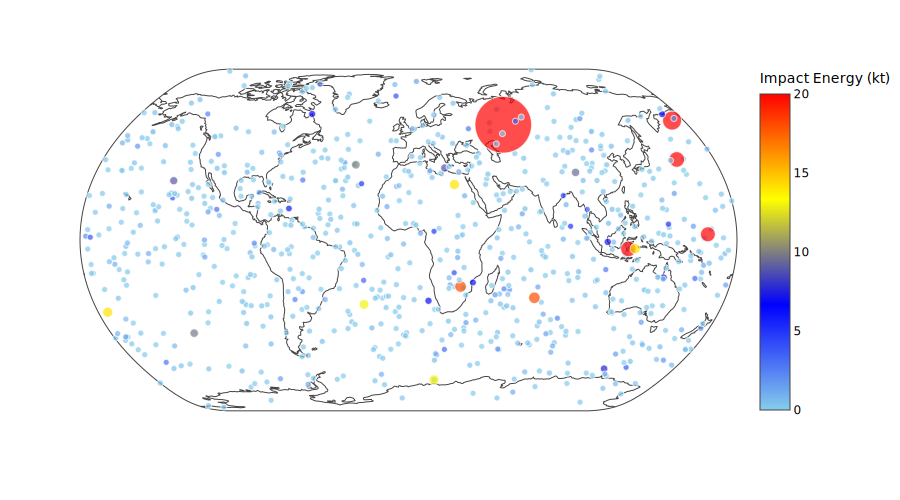
\includegraphics[width=\linewidth]{fireballs.png}
	\caption{Fireballs reported by US government sensors from April 15, 1988, to May 15, 2024. The size and color of each circle were determined by the logarithm of the impact energy (kt), and the location was determined by the altitude and longitude. All this data was obtained from the database published by NASA’s CNEOS at JPL.}
	\label{fig:fireballs}
\end{figure*}

At first, the covariance matrix was used to find the linear bond between NEOs' absolute magnitude ($H$)
and impact probability, but due to the correlation not being linear, it was discarded. Then proceeded
to use Pearson's and Spearman's correlation coefficients to analyze better the data and determine if a
correlation existed and which type it was.

At last, using Gnuplot and Python with various libraries such as pandas, numpy, plotly, a graphic
representation of geographic locations with their respective impact energy as the size of the reported
events was made.

%------------------------------------------------
\section{Results}

Here there goes the results

\begin{figure}[H] % Single column figure
	\includegraphics[width=\linewidth]{fit.png}
	\caption{Histogram of the logarithm of fireballs' impact energy ($kt$) reported by US government sensors from April 15, 1988, to May 15, 2024. The red line indicates the fit of a Gaussian distribution that was applied to the data. The larger impact energy was of $6\:log(kt)$.}
	\label{fig:gaussian}
\end{figure}

\begin{figure}[H] % Single column figure
	\includegraphics[width=\linewidth]{correlation.png}
	\caption{Plot between NEOs' impact probability and absolute magnitude ($H$) obtained from the database published by NASA’s CNEOS at JPL. The olive line indicates an exponential fit and the yellow one indicates a logarithmic fit, both were applied to the data.}
	\label{fig:probability}
\end{figure}

%------------------------------------------------

\section{Discussion}


%----------------------------------------------------------------------------------------
%	 REFERENCES
%----------------------------------------------------------------------------------------

\printbibliography % Output the bibliography

%----------------------------------------------------------------------------------------

\end{document}
